\providecommand{\main}{../../..}
\documentclass[\main/main.tex]{subfiles}
\begin{document}

\subsection{Esercizio 8}
Si determini la soluzione ottima supponendo che il decisore dichiari un tasso marginale di sostituzione uniforme di 4 unità di $f_1$ per una unità di $f_2$.

\begin{figure}
  \begin{align*}
    \max f_1 = x_1 -3x_2   \\
    \max f_2 = -4x_1 + x_2 \\
    -2x_1 + 2x_2 & \leq 7  \\
    2x_1 + 2x_2  & \leq 11 \\
    x_1          & \leq 4  \\
    x_1, x_2     & \geq 0
  \end{align*}
  \caption{Esercizio 8}
\end{figure}

\subsection{Soluzione esercizio 8}
\subsubsection*{Costruisco funzione obbiettivo}

\[
  u^* = f_1 + 4f_2 = x_1 -3x_2 + 4(-4x_1 + x_2) = -15x_1 + x_2
\]

\subsubsection*{Risolvo il problema lineare}
\begin{align*}
  \max -15x_1 + x_2      \\
  -2x_1 + 2x_2 & \leq 7  \\
  2x_1 + 2x_2  & \leq 11 \\
  x_1          & \leq 4  \\
  x_1, x_2     & \geq 0
\end{align*}
La variabile con coefficiente maggiore è la $x_1$ e ll valore minimo che essa può assumere è $0$, il valore massimo invece che può assumere la $x_2$ è $\frac{7}{2}$.

Il punto di ottimo risulta quindi: $(0, \frac{7}{2})$.

\begin{figure}
  \begin{subfigure}{0.45\textwidth}
    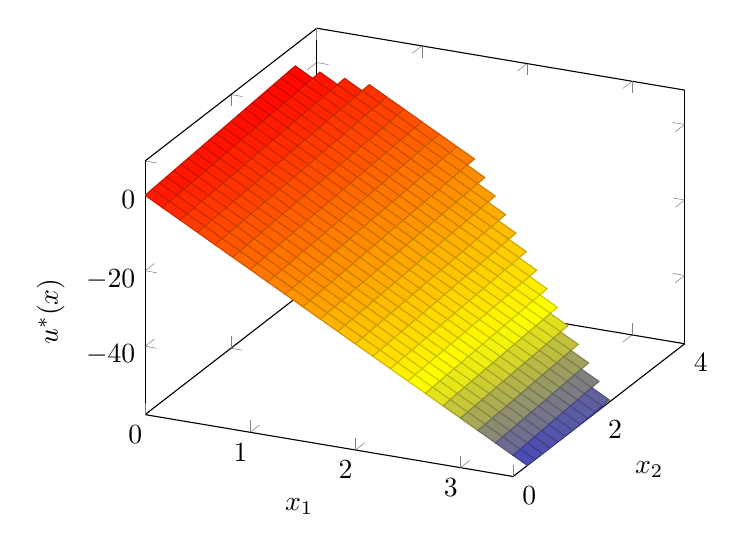
\begin{tikzpicture}
      \begin{axis}[
          xlabel=$x_1$,
          ylabel=$x_2$,
          zlabel=$u^*(x)$,
          domain=0:4,
          y domain=0:4,
          xmax=3.5
        ]
        \addplot3[surf, unbounded coords=jump]
        {-2*x+2*y<=7 && 2*x+2*y <= 11? -15*x + y: NaN};
      \end{axis}
    \end{tikzpicture}
    \caption{La funzione $u^*(x)$}
  \end{subfigure}
  ~
  \begin{subfigure}{0.45\textwidth}
    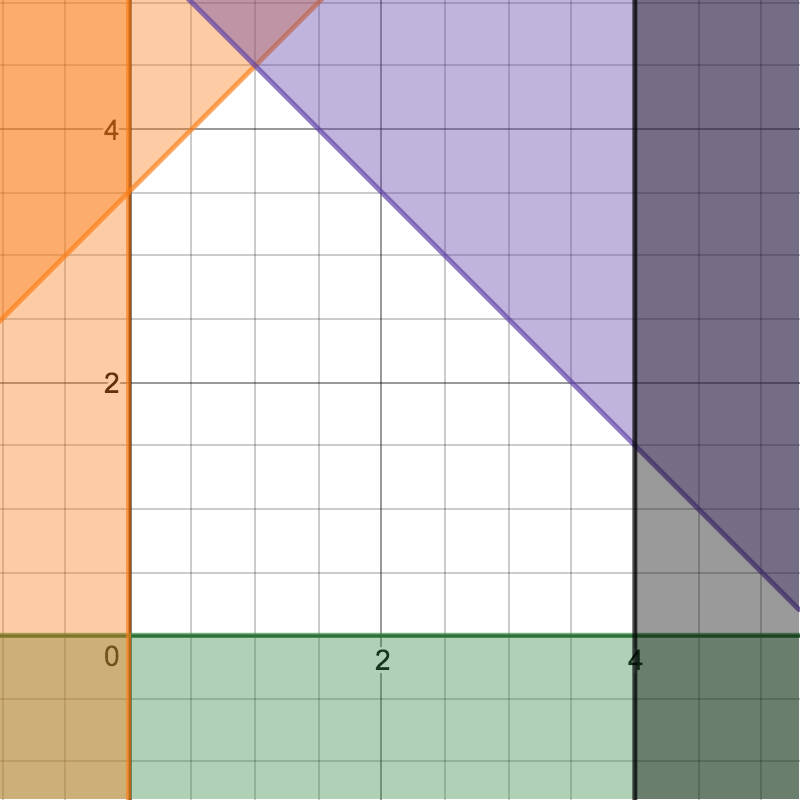
\includegraphics[width=0.8\textwidth]{es8-maut}
    \caption{Dominio della funzione $u^*(x)$}
  \end{subfigure}
\end{figure}
\end{document}